\documentclass[border=2pt]{standalone}
\usepackage{pgfplots}

\begin{document}
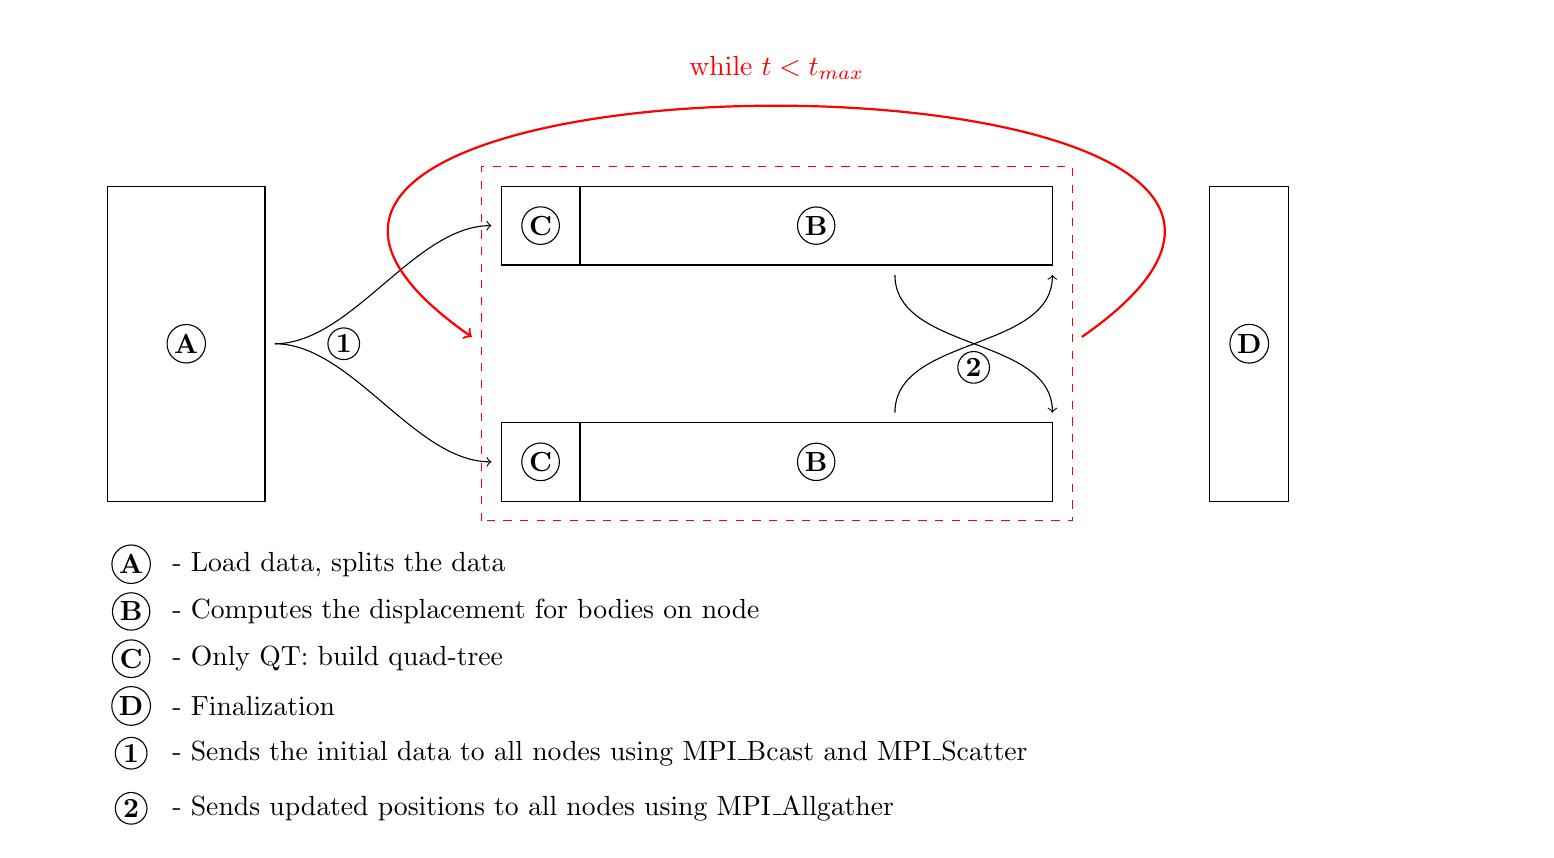
\begin{tikzpicture}
  \draw (0,-2) rectangle (2,2) node[draw,circle,inner sep=1pt,pos=0.5] {\textbf{A}};
  \node (split) at (2,0) {};

  \draw (6,1) rectangle (12,2) node[draw,circle,inner sep=1pt,pos=0.5] {\textbf{B}};
  \node (topEnd) at (12,1) {};
  \node (topStart) at (10,1) {};
  \node (topMiddleStart) at (5,1.5) {};
  \node (topMiddleEnd) at (12,1.5) {};

  \draw (5,1) rectangle (6,2) node[draw,circle,inner sep=1pt,pos=0.5] {\textbf{C}};
  \draw (5,-1) rectangle (6,-2) node[draw,circle,inner sep=1pt,pos=0.5] {\textbf{C}};

  \draw (6,-1) rectangle (12,-2) node[draw,circle,inner sep=1pt,pos=0.5] {\textbf{B}};
  \node (bottomEnd) at (12,-1) {};
  \node (bottomStart) at (10,-1) {};
  \node (bottomMiddleStart) at (5,-1.5) {};
  \node (bottomMiddleEnd) at (12,-1.5) {};

  \draw[->] (topStart) .. controls ++(90:-1.1) and ++(-90:-1.1) .. (bottomEnd);
  \draw[->] (bottomStart) .. controls ++(-90:-1.1) and ++(90:-1.1) .. (topEnd);

  \draw[->] (split) .. controls ++(180:-1.1) and ++(0:-1.1) .. (topMiddleStart);
  \draw[->] (split) .. controls ++(180:-1.1) and ++(0:-1.1) .. (bottomMiddleStart);



  \draw (14,-2) rectangle (15,2) node[draw,circle,inner sep=1pt,pos=0.5] {\textbf{D}};

  \draw[dashed, red] (4.75,-2.25) rectangle (12.25,2.25);
  \node (timeEnd) at (12.25,0) {};
  \node (timeStart) at (4.75,0) {};
  
  \draw[->, red, thick] (timeEnd) .. controls (18,4) and (-1,4) .. (timeStart);
  \node[red] (timeLabel) at (8.5,3.5) {while $t < t_{max}$};
  \node[draw,circle,inner sep=1pt] (splitLabel) at (3,0) {\textbf{1}};
  \node[draw,circle,inner sep=1pt] (splitLabel) at (11,-0.3) {\textbf{2}};

  % Labeling \node[draw,circle,inner sep=1pt] at (0.3,-2.6)
  \node[draw,circle,inner sep=1pt] at (0.3,-2.8) {\textbf{A}};
  \node[draw,circle,inner sep=1pt] at (0.3,-3.4) {\textbf{B}};
  \node[draw,circle,inner sep=1pt] at (0.3,-4.0) {\textbf{C}};
  \node[draw,circle,inner sep=1pt] at (0.3,-4.6) {\textbf{D}};
  \node[draw,circle,inner sep=1pt] at (0.3,-5.2) {\textbf{1}};
  \node[draw,circle,inner sep=1pt] at (0.3,-5.9) {\textbf{2}};

  \node[right] at (0.7,-2.8) {- Load data, splits the data};
  \node[right] at (0.7,-3.4) {- Computes the displacement for bodies on node};
  \node[right] at (0.7,-4.0) {- Only QT: build quad-tree};
  \node[right] at (0.7,-4.6) {- Finalization};
  \node[right] at (0.7,-5.2) {- Sends the initial data to all nodes using MPI\_Bcast and MPI\_Scatter};
  \node[right] at (0.7,-5.9) {- Sends updated positions to all nodes using MPI\_Allgather};

\end{tikzpicture}
\end{document}
